% id: 0600
% book: RPM 대수 · 06 삼각함수의 그래프
% section: 유형 06 그래프가 주어진 삼각함수의 미정계수 구하기
% figure: crop:fig-0600.png
% answer: $30$
% answer_source: 답지
% variant_level: 0 (원본 전사)
% 이 파일은 build.mjs 가 items.json 에서 만든다. 고칠 때는 items.json 을 고친다.
\smash{\raisebox{4.5mm}{\dmkichul{RPM 대수 0600번 · 80쪽}}}
\noindent\begin{minipage}[t]{0.58\linewidth}\vspace{0pt}\raggedright 함수 $y=a\cos\dfrac{\pi}{6}(2x+1)+b$의 그래프가 오른쪽 그림과 같을 때, 상수 $a$, $b$, $c$에 대하여 $abc$의 값을 구하시오. \cond{$a>0$}\end{minipage}\hfill\begin{minipage}[t]{0.4\linewidth}\vspace{0pt}\centering \setlength{\dmfigw}{104.6pt}\ifdim\dmfigw>\linewidth\setlength{\dmfigw}{\linewidth}\fi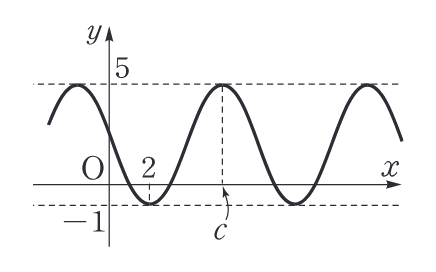
\includegraphics[width=\dmfigw]{figures/fig-0600.png}\end{minipage}\par
